
%(BEGIN_QUESTION)
% Copyright 2009, Tony R. Kuphaldt, released under the Creative Commons Attribution License (v 1.0)
% This means you may do almost anything with this work of mine, so long as you give me proper credit

Examine this portion of a P\&ID.  This particular diagram shows some of the piping and instrumentation associated with a chemical reactor vessel:

$$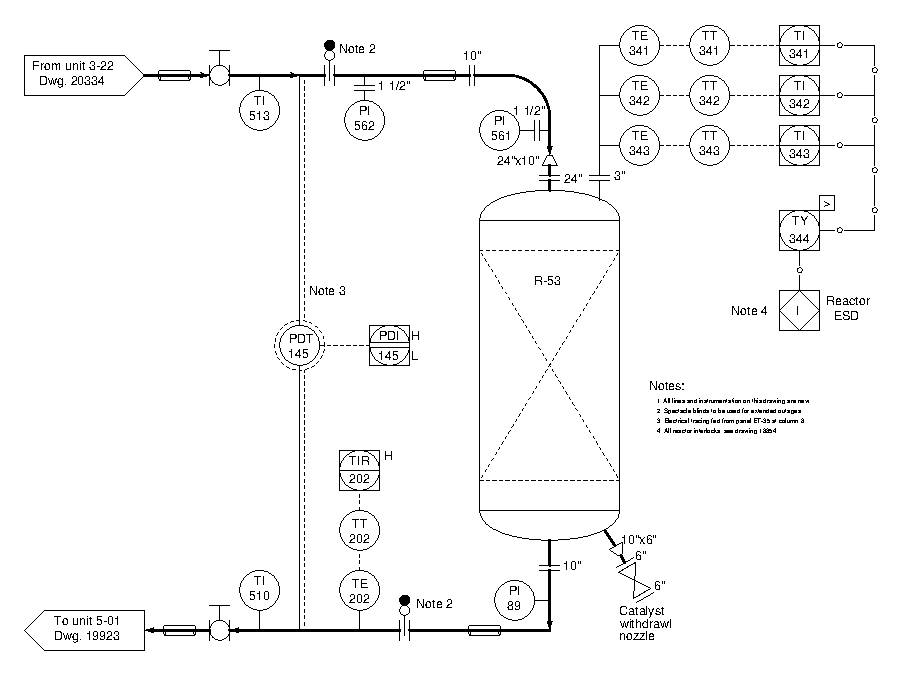
\includegraphics[width=15.5cm]{i03890x01.eps}$$


\begin{itemize}
\item{} Which direction does process fluid flow through this reactor vessel?  How can we tell from the diagram?
\vskip 10pt
\item{} Identify the functions of all instrument ``bubbles'' shown in this diagram, as well as the meanings of their identifying tag letters (e.g. ``PDT'').
\vskip 10pt
\item{} How are piping {\it flanges} shown in a PFD or P\&ID?
\vskip 10pt
\item{} What is the meaning of the trapezoidal symbols with two sizes (e.g. 10" $\times$ 24")?
\vskip 10pt
\item{} Two places on this diagram show the placement of a {\it blind}, used to positively seal off a pipe at a flange for maintenance purposes.  Locate these two blind installations in the diagram.
\vskip 10pt
\item{} Some of the indicators shown in this P\&ID serve double-duty as process alarms.  Identify which of the indicators also have alarm functions, and which of those are high alarms, low alarms, or both.
\end{itemize}

\vskip 20pt \vbox{\hrule \hbox{\strut \vrule{} {\bf Suggestions for Socratic discussion} \vrule} \hrule}

\begin{itemize}
\item{} Based on what you see in this P\&ID, what do you think the purpose of PDT-145 is?
\item{} Based on what you see in this P\&ID, what do you think is the purpose of having {\it three} temperature transmitters at the top of the vessel?
\item{} How are additional documents cross-referenced within this P\&ID?
\item{} Are there sections of your textbook that might be helpful to you in understanding this P\&ID which were not explicitly assigned for reading?
\end{itemize}

\underbar{file i03890}
%(END_QUESTION)





%(BEGIN_ANSWER)

If a blind or another other safety device needs to be left in its safe state for any specific reason, the person engaging that safety device must {\it lock} it in place and {\it tag} it with an informative tag stating the reason and duration of the lock-out.  This is commonly referred to as a {\it lock-out}, {\it tag-out} procedure.

%(END_ANSWER)





%(BEGIN_NOTES)

Process flow is top to bottom (follow the arrows).

\vskip 10pt

PDT = Differential pressure transmitter

TE = Temperature element (sensor)

PI = Pressure indicator

TY = Temperature relay/converter/computing function

\vskip 10pt

Pipe flanges shown by short parallel lines perpendicular to the pipe.

\vskip 10pt

Trapezoid = pipe reducer/expander, with pipe sizes specified

\vskip 10pt

Blinds have ``Note 2'' near them.

\vskip 10pt

Process alarms indicated by ``H'' (high) and ``L'' (low) letters written next to the instrument bubble symbols.

\vskip 10pt














\vskip 20pt \vbox{\hrule \hbox{\strut \vrule{} {\bf Virtual Troubleshooting} \vrule} \hrule}

This question is a good candidate for a ``Virtual Troubleshooting'' exercise.  Presenting the diagram to students, you first imagine in your own mind a particular fault in the system.  Then, you present one or more symptoms of that fault (something noticeable by an operator or other user of the system).  Students then propose various diagnostic tests to perform on this system to identify the nature and location of the fault, as though they were technicians trying to troubleshoot the problem.  Your job is to tell them what the result(s) would be for each of the proposed diagnostic tests, documenting those results where all the students can see.

During and after the exercise, it is good to ask students follow-up questions such as:

\begin{itemize}
\item{} What does the result of the last diagnostic test tell you about the fault?
\item{} Suppose the results of the last diagnostic test were different.  What then would that result tell you about the fault?
\item{} Is the last diagnostic test the best one we could do?
\item{} What would be the ideal order of tests, to diagnose the problem in as few steps as possible?
\end{itemize}


%INDEX% Process: chemical reactor (realistic P&ID shown)

%(END_NOTES)


